\documentclass[10pt]{article}
\usepackage{icmlko}

\icmlmeta{IP 파운데이션 월드모델}{124}{축이 비어 있었다}{노트 123의 ``주최자 주장은 신호가 아니다''를 정정한다 --- 그 247건은 열 축이 전부 상수 2.0이다. 사람이 안 매겼을 뿐이고, 매기면 스물한 해가 한 번의 작업이 된다}

\begin{document}

\twocolumn[
\icmlheader

\begin{abstract}
노트 123이 주최자 주장 라벨을 넣으면 팝업 $\rho$가 $+$0.4601에서 $+$0.0352로
무너지는 것을 보고 \textbf{``주최자 주장 방문자 수에는 예측 가능한 신호가
없다''}고 적었다. \textbf{틀렸다.} 그 결론을 확인하려고 축 분포를 비교하다
이상한 것을 봤다 --- 열 축의 상관이 전부 정확히 같은 값으로 나왔다. 파 보니
답이 하나였다. \textbf{주최자 주장 247건은 열 축이 전부 상수 2.0이다.}
사람이 기획서를 읽고 매긴 적이 없고 중립값으로 채워져 있다. 언론 추정 13건도
같다. 계수 방법별로 세면 갈린다 --- 입장 54 · 참여 37 · 미상 20 · 노출 5는
\textbf{상수인 축이 0개}이고, 주최자 주장 247 · 언론 추정 13은
\textbf{10개 전부}다. \textbf{그러므로 노트 123이 잰 것은 라벨의 질이 아니라
빈 칸이었다.} 축이 전부 같으면 어떤 모형도 순위를 못 매기므로 $\rho\approx0$
이 나올 수밖에 없다. \textbf{그리고 이것이 노트 123의 결론을 뒤집는다.}
발굴이 막힌 것이 아니라 \textbf{매기면 된다.} 라벨은 이미 있다 --- 376건 중
축이 매겨진 것이 116건, 빈 것이 260건이다. 축을 매겨 322건이 되면 구간 반폭이
0.0509에서 \textbf{0.0141}로 준다. 노트 123이 ``스물한 해''라 한 것이
\textbf{한 번의 태깅 작업}이 된다. \textbf{다만 라벨의 질은 여전히 미검정이다}
--- 주최자 주장이 실측과 얼마나 다른지는 축을 매긴 뒤에야 잴 수 있다.
\end{abstract}
]

\begin{figure*}[t]
\centering
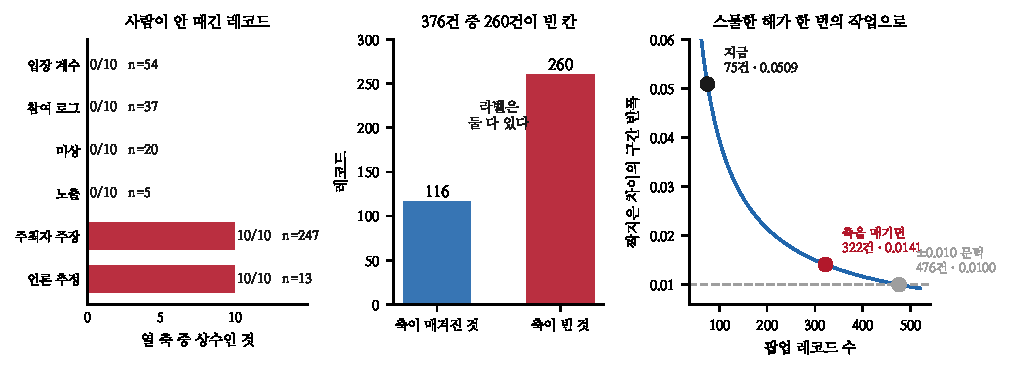
\includegraphics[width=\textwidth]{figs/em.pdf}
\caption{왼쪽 --- 사람이 안 매긴 레코드. 가운데 --- 376건 중 260건이 빈 칸.
오른쪽 --- 스물한 해가 한 번의 작업으로.}
\end{figure*}

\section{이상한 것을 봤다}

노트 123의 결론을 확인하려고 부풀림이 어느 축과 붙는지 쟀다. 열 축의 상관이
\textbf{전부 정확히 $+$0.207}로 나왔다. 그런 일은 없다.

\begin{table}[t]
\centering\tsize
\caption{계수 방법별로 열 축 중 상수인 것.}
\begin{tabular}{lrr}
\toprule
& $n$ & 상수인 축 \\
\midrule
입장 계수 & 54 & \textbf{0/10} \\
참여 로그 & 37 & \textbf{0/10} \\
미상 & 20 & \textbf{0/10} \\
노출 & 5 & \textbf{0/10} \\
\midrule
\textbf{주최자 주장} & \textbf{247} & \textbf{10/10} \\
\textbf{언론 추정} & \textbf{13} & \textbf{10/10} \\
\bottomrule
\end{tabular}
\end{table}

\claimx{\textbf{주최자 주장 247건과 언론 추정 13건은 열 축이 전부 상수
2.0이다} --- 0$\sim$4 눈금의 한가운데다. 사람이 기획서를 읽고 매긴 적이 없고
중립값으로 채워져 있다.}{왜 2.0으로 채웠는지는 자료에 안 적혀 있다. 결과보고서
발굴 때 라벨만 뽑고 기획서 태깅은 안 한 것으로 보이는데 확인 못 했다.}

\section{그래서 노트 123이 잰 것은 빈 칸이었다}

축이 전부 같으면 어떤 모형도 순위를 못 매긴다. 노트 123의 세 수치가 다시
읽힌다.

\begin{table}[t]
\centering\tsize
\caption{노트 123의 수치와 그 뜻.}
\begin{tabular}{lrl}
\toprule
& $\rho$ & 실제로 뜻하는 것 \\
\midrule
실측만 & $+$0.4601 & 축이 매겨진 75건 \\
$+$주최자 주장 & $+$0.0352 & 98건이 빈 칸으로 섞임 \\
주최자 주장만 & $-$0.0539 & \textbf{전부 빈 칸 --- 잴 것이 없다} \\
\bottomrule
\end{tabular}
\end{table}

\claimx{\textbf{노트 123의 ``주최자 주장은 신호가 아니었다''를 정정한다.}
잰 것은 라벨의 질이 아니라 축의 부재다. \textbf{주최자 주장 라벨의 질은
아직 검정되지 않았다.}}{노트 123의 다른 결론들 --- 구간 축소 법칙
$2.28\,n^{-0.88}$, 필요 표본 476건, 관문 폭포 --- 은 그대로다. 축이 매겨진
75건만 쓴 계산이기 때문이다.}

\section{발굴이 막힌 것이 아니었다}

\begin{table}[t]
\centering\tsize
\caption{376건의 실제 상태.}
\begin{tabular}{lrl}
\toprule
축이 매겨진 것 & \textbf{116} & 그중 관문 통과 75 \\
축이 빈 것 & \textbf{260} & 라벨은 있다 \\
\bottomrule
\end{tabular}
\end{table}

\begin{table}[t]
\centering\tsize
\caption{축을 매기면 구간이 이렇게 준다.}
\begin{tabular}{lrr}
\toprule
& $n$ & 반폭 \\
\midrule
지금 & 75 & 0.0509 \\
미상 · 노출까지 & 100 & 0.0395 \\
\textbf{주최자 주장까지} & \textbf{322} & \textbf{0.0141} \\
전부 & 376 & 0.0123 \\
\midrule
$\pm$0.010 문턱 & 476 & 0.0100 \\
\bottomrule
\end{tabular}
\end{table}

\claimx{\textbf{노트 123이 ``스물한 해''라 한 것이 한 번의 태깅 작업이 된다.}
라벨은 이미 있고 축만 비어 있다. 322건이 되면 반폭이 0.0141로 지금의 3분의
1이 되고, $\pm$0.010 문턱까지 154건만 더 남는다.}{\textbf{라벨의 질이
미검정이다.} 주최자 주장이 실측과 체계적으로 다르면 표본을 늘려도 편향만
늘어난다. 축을 매긴 뒤 두 부분집합을 견줘야 안다 --- \textbf{그것이 이 작업의
첫 산출물이어야 한다.}}

\begin{quote}\fontsize{9.5}{11.5}\selectfont
노트 116이 ``재지 말고 걸어 봐라''로 바꾼 뒤 노트 117이 누수를, 노트 119가
정합을, 그리고 이 노트가 빈 칸을 잡았다. \textbf{검정이 싸지면 자료의 결함이
성능 수치로 위장해서 들어온다.} 세 번 다 ``수치가 이상하다''가 아니라
``수치가 너무 깔끔하다''가 단서였다 --- 채택 4/4, 완벽한 분리, 열 축이 같은 값.
\end{quote}

\section{한계}

\begin{itemize}[leftmargin=1.1em,itemsep=0.15em]
\item \textbf{채택할 것이 없다.} 이 노트는 정정이지 개선이 아니다.
\item 왜 2.0으로 채웠는지 자료에 안 적혀 있다.
\item \textbf{주최자 주장 라벨의 질은 여전히 미검정이다.} 축을 매기기 전에는
      못 잰다.
\item 322건 반폭 0.0141은 외삽이다. 새로 매긴 축의 질이 지금 것과 같다는
      가정이 들어간다.
\item 노트 123의 제목과 요약이 틀린 채로 나갔다. 이 노트가 정정이다.
\end{itemize}

\section{다음}

\begin{enumerate}[leftmargin=1.3em,itemsep=0.15em]
\item \textbf{태깅 지침을 한 장으로 쓴다} --- 기획서에서 열 축을 매기는 규칙.
      이미 매겨진 116건이 훈련 예제가 된다.
\item \textbf{먼저 스무 건만 매겨 라벨의 질을 잰다} --- 주최자 주장 중 스무
      건에 축을 매기고, 실측 75건으로 배운 모형이 그것들을 맞히는지 본다.
      \textbf{맞히면 247건을 다 매길 값이 있고, 안 맞히면 라벨이 문제다.}
\item \textbf{자동 태깅을 검토한다} --- 기획서 텍스트에서 축을 뽑는 것.
      116건이 지도 자료다.
\item 노트 122가 남긴 도구 문서 고치기.
\end{enumerate}

\vspace{0.6em}
\hrule height 0.3pt
\vspace{0.5em}
{\footnotesize
\textbf{참고문헌}\\[0.3em]
Kaufman, S. et al. (2012). Leakage in data mining: formulation, detection, and
avoidance. \emph{ACM TKDD}, 6(4), 1--21.\\[0.15em]
Little, R. J. A., Rubin, D. B. (2019). \emph{Statistical Analysis with Missing
Data}, 3rd ed. Wiley.\\[0.15em]
Varoquaux, G. (2018). Cross-validation failure: small sample sizes lead to large
error bars. \emph{NeuroImage}, 180, 68--77.\\[0.15em]
Efron, B., Tibshirani, R. J. (1993). \emph{An Introduction to the Bootstrap}.
Chapman \& Hall.\\[0.15em]
Halevy, A., Norvig, P., Pereira, F. (2009). The unreasonable effectiveness of
data. \emph{IEEE Intelligent Systems}, 24(2), 8--12.
}

\end{document}
